%!TEX root = ../Studienarbeit.tex

\chapter{Umsetzung}

\section{Softwareentwicklung}
In diesem Abschnitt der Studienarbeit wird die Auswahl des Mikrocontrollers erklärt und das Zusammenspiel der Softwarekomponenten sowie einige Kernkomponenten detaillierter beschrieben.

\subsection{Auswahl der Mikrocontrollers}
Als Mikrocontroller wird das kostengünstige ESP32-WROOM-32E-Modul -- zirka 5~€ \cite{espressifModules} -- verwendet, da es in Hobbyprojekten gern verwendet wird \cites{redditESP32}{esp32Forum}. Folglich gibt es eine große Community, die sich bei Problemen während der Entwicklung von Softwareprojekten austauschen kann \cites{redditESP32}{esp32Forum}. Die \ac{ESP-IDF} ist außerdem gut durch Kommentare im Sourcecode und durch Beispielprogramme dokumentiert. Ein weiterer Grund für die Verwendung des ESP32 ist, die Unterstützung mehrerer Bluetooth-Stacks, welche in Kapitel \ref{section:bluetoothStacks} beschrieben sind. Zuletzt ist noch anzumerken, dass der Mikrocontroller in kompakten Hardwaremodulen bezogen werden kann, in denen alle benötigten Elektronikkomponenten für den Betrieb des ESP32 enthalten sind. Dazu zählen unter anderen Kondensatoren, Widerstände und gegebenenfalls eine Antenne für den Betrieb von Bluetooth oder \acs{WLAN} \cite[S.~14]{espressifHardwareDesignGuidelines}. Die ESP32-Module besitzen auch meist eine CE-Zertifizierung, wie in Kapitel \ref{section:esp32Explained} beschrieben, womit das zu entwickelnde Fernsteuerungsmodul vereinfacht zertifiziert werden kann.

\subsection{Auswahl des Bluetooth-Stacks}
\label{section:bluetoothStackSelection}
Da die Kommunikation zwischen dem Fernsteuerungserweiterungsmodul und den Endgeräten mittels \ac{BLE} erfolgen soll, wird der Bluetooth-Stack Apache NimBLE verwendet. Dieser wird bei der ausschließlichen Verwendung von \ac{BLE} empfohlen, da er eine geringe Codegröße hat und wenig Speicher zu Laufzeit benötigt \cite{espidfBluetoothStack}.

\subsection{Kommunikation zwischen dem Mikrocontroller und dem Endgerät}
\label{section:communicationModuleDevice}
Für die Übermittlung der Daten zwischen dem Mikrocontroller zu einem Endgerät wird \ac{BLE} verwendet, indem die Fernsteuerungsdaten mittels \ac{HOGP} verpackt werden. \ac{BLE} eignet sich, wie im Kapitel \ref{section:bluetoothGenerall} beschrieben, gut durch den geringen Stromverbrauch, da das Fernsteuerungsmodul durch den Akku der Fernsteuerung mitbetrieben wird. Die Verwendung des \ac{HID}-Datenformats ermöglicht dem Erweiterungsmodul, Daten für die Steuerung von Simulatoren an viele Endgeräte ohne zusätzlich benötigte Treiber zu übertragen \cite{microsoftHID}. Für die Datenübertragung werden die \ac{BLE}-Dienste und Merkmale, welche in Tabelle \ref{table:usedServicesAndCharacteristics} zu sehen sind, verwendet. Zusätzlich enthält das Report-Merkmal einen Konfigurationsdeskriptor, womit sich Endgeräte für das automatische versenden von Daten abonnieren können.

\begin{longtable}[c]{|l|l|}
    \caption{Liste der verfügbaren Geräteinformationsmerkmale}
    \label{table:usedServicesAndCharacteristics}\\
    \hline
    \textbf{\ac{BLE}-Dienst} & \textbf{Merkmale}\\
    \hline
    \hline
    \endfirsthead

    \hline
    \textbf{\ac{BLE}-Dienst} & \textbf{Merkmale}\\
    \hline
    \hline
    \endhead

    \hline
    \multicolumn{2}{|r|}{Weitere \ac{BLE}-Dienste auf der nächsten Seite}\\
    \hline
    \endfoot

    \hline
    \endlastfoot
    
    \multirow{4}{*}{Geräteinformationsdienst} & Herstellername\\
    \cline{2-2}
     & Modellnummer\\
     \cline{2-2}
     & Firmwareversion\\
     \cline{2-2}
     & Softwareversion\\
    \hline
    \multirow{1}{*}{Batteriedienst} & Akkustand\\
    \hline
    \multirow{4}{*}{\ac{HID}-Dienst} & Report-Map\\
    \cline{2-2}
     & \ac{HID} Information\\
     \cline{2-2}
     & \ac{HID} Control Point\\
     \cline{2-2}
     & Report, definiert als Eingabe\\
\end{longtable}

Der finale Report-Map-Deskriptor ist für die Übertragung von Gamepaddaten konfiguriert. Diese Daten bestehen dafür aus acht analogen und acht digitalen Kanaldaten, welche jeweils die absoluten Stellungen der Fernsteuerungseingaben wiedergeben. Die analogen Kanäle haben eine Größe von 16~Bit und einen Wertebereich von 0 bis 2047. Die ersten vier analogen Kanäle werden für die Übertragung der Steuerknüppelpositionen verwendet. Die restlichen vier analogen Kanäle werden für die Stellung der Kippschalter mit jeweils drei Positionen verwendet. Die digitalen Kanäle haben jeweils eine Größe von 1~Bit und werden für Knöpfe mit 2 Stellungen benutzt. In Quellcode \ref{lst:reportDescriptorModule} ist der beschriebene Report Deskriptor zu sehen.

Damit das Erweiterungsmodul von Endgeräten als Gamepad während des Verbindungsaufbaus erkannt wird, enthalten die Advertising-Pakete ebenso Informationen über das Erweiterungsmodul.

\begin{lstlisting}[caption=Report Map Deskriptor des Erweiterungsmoduls, label={lst:reportDescriptorModule}, style=generalStyle]
    0x05, 0x01,        // Usage Page (Generic Desktop Ctrls)
    0x09, 0x05,        // Usage (Game Pad)
    0xA1, 0x01,        // Collection (Application)
    0x85, 0x01,        // Report Id (1)
    0xA1, 0x00,        //   Collection (Physical)
    0x05, 0x01,        //     Usage Page (Generic Desktop Ctrls)
    0x09, 0x30,        //     Usage (X)
    0x09, 0x31,        //     Usage (Y)
    0x09, 0x32,        //     Usage (Z)
    0x09, 0x33,        //     Usage (Rx)
    0x09, 0x35,        //     Usage (Rz)
    0x09, 0x34,        //     Usage (Ry)
    0x09, 0x36,        //     Usage (Slider)
    0x09, 0x36,        //     Usage (Slider)
    0x15, 0x00,        //     Logical Minimum (0)
    0x26, 0xFF, 0x07,  //     Logical Maximum (2047)
    0x75, 0x10,        //     Report Size (16)
    0x95, 0x08,        //     Report Count (8)
    0x81, 0x02,        //     Input (Absolute)
    0x05, 0x09,        //     Usage Page (Button)
    0x19, 0x01,        //     Usage Minimum (0x01)
    0x29, 0x08,        //     Usage Maximum (0x08)
    0x15, 0x00,        //     Logical Minimum (0)
    0x25, 0x01,        //     Logical Maximum (1)
    0x95, 0x08,        //     Report Count (8)
    0x75, 0x01,        //     Report Size (1)
    0x81, 0x02,        //     Input (Absolute)
    0xC0,              //   End Collection
    0xC0,              // End Collection
\end{lstlisting}

Zusätzlich zu den in Kapitel \ref{section:appleAnforderungen} beschriebenen Sollanforderungen durch Apple haben Geräte von Apple weitere nicht dokumentierte Anforderungen. Zum Beispiel muss das Erweiterungsmodul \ac{RPA} auflösen können, da sonst kein Verbindungsaufbau zum Datenaustausch zwischen den Geräten stattfindet. Eine weitere nicht dokumentierte Anforderung ist die verschlüsselte Datenübertragung zwischen dem Erweiterungsmodul und dem Applegerät, wenn es sich um \ac{HID}-Daten handelt. Dafür werden im ersten Schritt die Geräte gekoppelt, was durch verschiedene Verfahren erfolgen kann. Die Kopplung mit dem Erweiterungsmodul findet durch die Anzeige und der Bestätigung eines Pins auf beiden Geräten statt. Im zweiten Schritt erfolgt das Bonding, womit die Daten der Kopplung gespeichert werden, um bei einem erneuten Verbindungsaufbau die Kopplungsphase zu überspringen \cite{kyneticsBondingPairng}.

Für die Ermittlung des aktuellen Verbindungszustands mit Endgeräten werden die auftretenden \ac{GAP}-Evente am Erweiterungsmodul ausgewertet. Ein verwendetes \ac{GAP}-Event ist für die Kopplung der Geräte zuständig und enthält die Erstellung und Darstellung des Kopplungspins. Ein weiteres \ac{GAP}-Event ist für das Abonnieren von Endgeräten zu \ac{BLE}-Merkmalen zuständig. Zuletzt wird das \ac{GAP}-Event für den Verbindungsaufbau verwendet, um eine Anfrage an das Endgerät zu schicken, damit die Übertragungsrate für die Verbindung erhöht wird.

\subsection{Kommunikationsprotokoll zwischen der Multikopterfernsteuerungen und dem Mikrocontroller}
\label{section:communicationCRSF}
Als Kommunikationsprotokoll zwischen der Multikopterfernsteuerung und dem Mikrocontroller wird CRSF verwendet, da wie in Kapitel \ref{section:communicationsProtocollsRemote} beschrieben das Protokoll die höchste Übertragungsrate bei möglichst kleinen Datenpaketen hat.

Da die CRSF-Daten mittels einer \ac{UART}-Verbindung übertragen werden, findet das Auslesen der Daten auf dem ESP32 mittels eines \ac{UART}-Treibers statt. Der \ac{UART}-Treiber abstrahiert dafür den vorhandenen \ac{UART}-Interrupt und stellt alle Ereignisse und Daten durch eine vereinfachte \ac{API} bereit \cite{espUARTDriver}. Der \ac{UART}-Interrupt ist konfiguriert, dass empfange Daten erst verarbeitet werden, wenn entweder der interne \ac{UART}-Buffer voll ist oder ein definierter Timeout zwischen empfangenen Bytes auftritt.

Die Auswertung der empfangenen CRSF-Daten findet in zwei Schritten statt. Im ersten Schritt findet eine Überprüfung der Geräteadresse -- 0xEE --, der Länge der übermittelten Daten und des übermittelten Datentyps -- 0x16 -- statt. Wenn all diese Werte stimmen findet die Überprüfung der \ac{CRC}-Prüfsumme statt, um festzustellen, ob alle Kanaldaten gültig sind. Im zweiten Schritt, werden alle Kanaldaten zunächst ausgelesen und darauffolgend im Wertebereich angepasst, damit der vollständige Wertebereich des \ac{HID}-Reports verwendet wird. Für die Anpassung des Wertebereichs werden die analogen Kanaldaten auf einen Wertebereich von 0 bis 2047 erweitert und digitale Kanaldaten bis zu einem Wert von 992 als logisch 0 und ab einen Wert von 993 als logisch 1 ausgewertet. Nach Anpassung des Wertebereichs werden die Daten in einer globalen Datenstruktur abgelegt, welche in Quellcode \ref{lst:channelDataStruct} zu sehen ist. Falls dabei eine Änderung des Wertes stattfindet, wird veranlasst, dass die Daten per \ac{BLE} an abonnierte Endgeräte versendet werden. Falls ein Problem während der Auswertung stattfindet, wird das komplette Paket verworfen und auf ein neues Paket gewartet.

\begin{lstlisting}[caption=C-Strukuraufbau der aufbereiteten Kanaldaten, label={lst:channelDataStruct}, style=generalStyle]
    typedef struct ChannelDataStruct{
        uint16_t roll;        //roll = x
        uint16_t pitch;       //pitch = y
        uint16_t aux3;        //aux3 = z
        uint16_t yaw;         //yaw = rx
        uint16_t aux1;        //aux1 = rz
        uint16_t throttle;    //throttle = ry
        uint16_t aux4;        //aux4 = slide
        uint16_t aux2;        //aux2 = slide
        uint8_t buttons;      //buttons = aux12(b8) .. aux5(b1)
    } ChannelDataStruct;
\end{lstlisting}

\subsection{Statusausgabe des Mikrocontrollers mittels eines \acs{OLED}-Displays}
\label{section:oledOutput}
Wie in Kapitel \ref{section:softwareRequirement} beschrieben, wird ein \acs{OLED}-Display verwendet, um Statusinformationen für den Benutzer darzustellen. Dabei hat das Display eine Displaydiagonale von 0,91~Zoll, eine Auflösung von 128 zu 32~Pixel und den Displaycontroller SSD1306. Die Datenübertragung zwischen dem ESP32 und dem SSD1306 findet mittels \ac{I2C} statt. Zur Ansteuerung einzelner Pixel im Display teilt der Displaycontroller das Display in vier Seiten mit jeweils 128 Segmenten auf. Jedes Segment hat dabei eine Größe von 8~Bit. Zu sehen ist die Aufteilung des Displays in Seiten und Segmente sowie die Pixelansteuerung durch einen übermittelten Datenstream in Abbildung \ref{fig:ssd1306PixelControl}.

\begin{figure}[h]
    \centering
    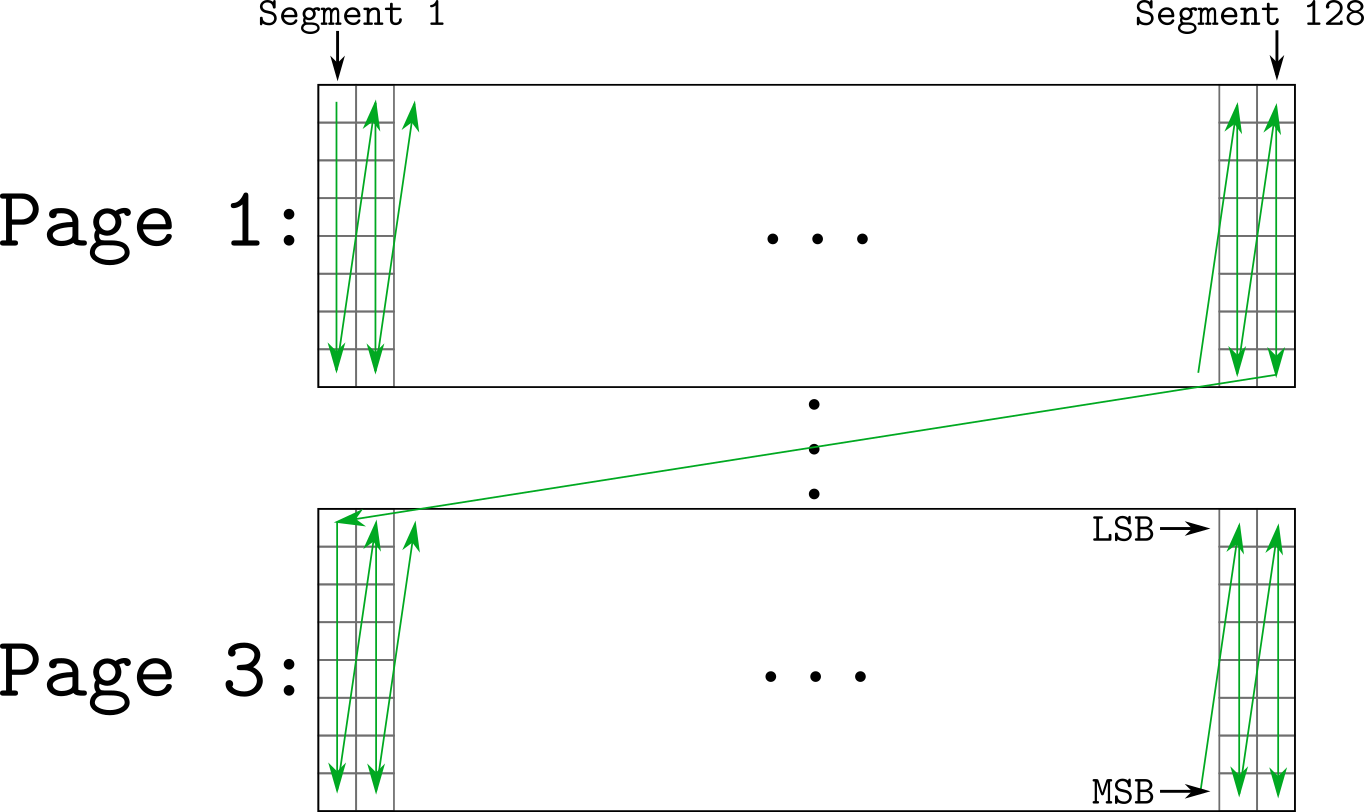
\includegraphics[width=.7\textwidth]{ssd1306}
    \caption{Verarbeitung eines Datenstreams für die Darstellung auf dem Erweiterungsmoduldisplay; abgewandelt von \cite[S.~37]{ssd1306}}
    \label{fig:ssd1306PixelControl}
\end{figure}

Die Darstellung von Text auf dem Display erfolgt mittels einer Bitmap-Schriftart, da dadurch mit geringerem Rechenaufwand eine gute Lesbarkeit auf dem kleinen Display erreicht wird. Alle Glyphen der Schriftart werden in einem zweidimensionalen Array gespeichert und haben eine Höhe von 14 und eine Breite von 9 Pixel. Die Umwandlung von Zeichenketten in Glyphen für das Display findet in zwei Schritten statt. Im ersten Schritt werden alle Pixelinformationen für das komplette Displaybild in einen lokalen 492~Byte großen Buffer des ESP32 zwischengespeichert. Jedes Bit dieses Buffers repräsentiert dabei ein Pixel des Displays. Dadurch müssen die Glypheninfromation aus dem zweidimensionalen Glyphenarray nur an die richtige Position des Buffers übertragen werden. Im zweiten Schritt wird der lokale Puffer mittels \ac{I2C} an das Display für die Darstellung übertragen. Die Aufteilung der Darstellung in zwei Schritten hat den Vorteil, dass Inhalte auf dem Display ohne Artefakte überlappt werden können, was nicht möglich wäre, wenn nur die zu veränderten Pixel an das Display geschickt werden würden.

\subsection{Kombination aller Softwarekomponenten}
\label{section:softwareCombination}
Für die einfachere Integration von eigenen Softwarekomponenten mit bereits vorhandenen Bibliotheken wird für die Studienarbeit die Programmiersprache C verwendet, da eine Vielzahl an Bibliotheken und Beispielprogrammen in C geschrieben sind \cite{espressifIDF}. Die finale Software des Mikrocontrollers besteht aus fünf Komponenten, welche mittels FreeRTOS-Echtzeitkernel verwaltet werden. 

Die erste Komponente für die \ac{BLE}-Kommunikation und dem \ac{BLE}-Verbindungsaufbau läuft in einen FreeRTOS-Task (\ac{BLE}-Task). Die zweite Komponente läuft ebenso in einen FreeRTOS-Task und liest und verarbeit CRSF-Daten von der Multikoperfernsteuerung (CRSF-Task). Die dritte Komponente, welche als FreeRTOS Software Timer integriert ist, bestimmt den aktuellen Akkustand. Hierfür wird mittels des integrierten \ac{ADC} des ESP32 die aktuelle Spannung des Multikopterfernsteuerungsakkus bestimmt und in einen Prozentwert zwischen 0 und 100 umgewandelt. Dieser Akkustand wird durch \ac{BLE} an das Endgerät weitergeschickt. Die vierte Komponente der ESP32-Software ist für die Erkennung von Tasteneingabeevents zuständig. Die Erkennung von Tasteneingaben erfolgt dabei mittels eines FreeRTOS-Interrupts und die Weitergabe der Daten an ein Task mittels FreeRTOS-Queues. Die letzte Softwarekomponente des ESP32 ist für die Steuerung des Displays vorgesehen. Da Anzeigeänderungen am Display nur selten erfolgen und schnell abgearbeitet werden können, werden die Displayhilfsfunktionen innerhalb der zwei vorhandenen Tasks ausgeführt und nicht in einem zusätzlichen Task. Damit der ESP32-Mikrocontroller mit den zwei vorhandenen Kernen optimal ausgelastet wird, werden beide Tasks jeweils einem Kern fest zugewiesen. Dadurch blockieren sich die einzelnen Softwarekomponenten im Betrieb seltener.

Zur Abspeicherung der Multikopterfernsteuerungsdaten und zum Datenaustausch zwischen CRSF-Task und \ac{BLE}-Task werden globale Variablen verwendet. Die Mitteilung über das Auslesen neuer Multikopterfernsteuerungsdaten findet mit zwei Funktionen von NimBLE statt. Zum einen durch die Funktion \textit{ble\_hs\_mbuf\_from\_flat}. Mittels dieser Funktion werden die Fernsteuerungsdaten in einen internen \ac{BLE}-Buffer geschrieben. Zum anderen durch die Funktion \textit{ble\_gattc\_notify\_custom}. Mittels dieser Funktion werden alle gespeicherten Daten im \ac{BLE}-Buffer automatisch an alle abonnierten Endgeräte versendet.

\subsection{Weiterführende Informationen}
Der vollständige Sourcecode der Studienarbeit ist für weitere Details öffentlich unter nachfolgenden Link auffindbar: \url{https://github.com/SimLinkModule/ModuleSoftware}

\section{Platinenentwurf}
\label{section:pcbImplementation}
Wie in Kapitel \ref{section:pcbRequirement} beschrieben, soll eine Platine entwickelt werden, die alle benötigten Elektronikkomponenten des Erweiterungsmoduls enthält. Dadurch wird es möglich das Erweiterungsmodul kompakt, mobil und benutzerfreundlich zu verwenden. Dafür sind alle Elektronikkomponenten auf drei Platinen, wie in Abbildung \ref{fig:pcbs} zu sehen, untergebracht, womit für die Gehäuseerstellung eine größtmögliche Flexibilität realisiert wird. \textit{Platine 1} dient als Verbindungsglied zwischen der Multikoperfernsteuerung und dem ESP32-Mikrocontroller. Hierzu enthält diese Platine zum einen eine Buchsenleiste mit der dargestellten Pinbelegung wie in Abbildung \ref{fig:pinoutController} zu sehen ist. Zusätzlich ist eine \ac{ESD}-Schutzschaltung vorhanden, welche im Kapitel \ref{section:esdProtection} genauer beschrieben wird. Auf der \textit{Platine 2} befindet sich die Hauptkomponenten des Erweiterungsmoduls. Dazu zählen die Spannungsregulierung, der ESP32-Mikrocontroller und die Logik für das Beschreiben des ESP32 mit Programmdaten. Alle Eingabe- und Ausgabeelemente für die Benutzerinteraktionen befinden sich auf der \textit{Platine 3}.

\begin{figure}[h]
    \centering
    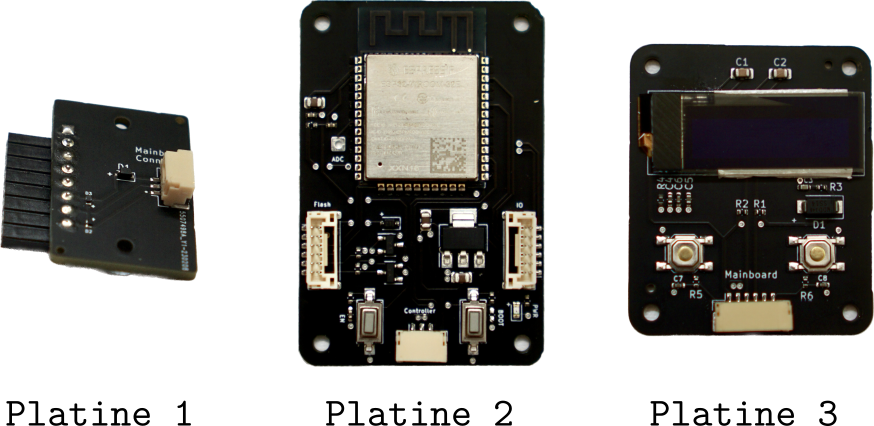
\includegraphics[width=.7\textwidth]{pcbs}
    \caption{Platinen des Erweiterungsmoduls}
    \label{fig:pcbs}
\end{figure}

\begin{figure}[h]
    \centering
    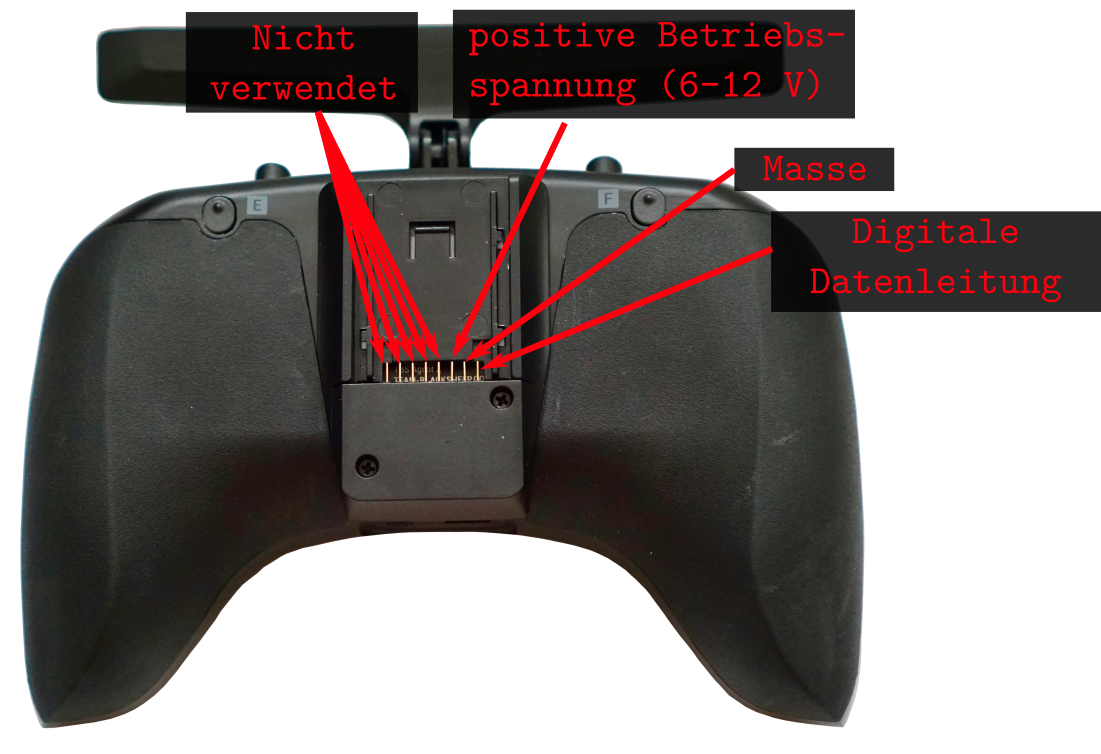
\includegraphics[width=.6\textwidth]{pinoutController}
    \caption{Pinbelegung des Fernsteuerungsmodulschachts; abgewandelt von \cite{liteModulePinout}}
    \label{fig:pinoutController}
\end{figure}

\subsection{Teilschaltungen}
In nachfolgenden Unterkapiteln werden die wichtigsten Teilschaltungen aller Platinen des Erweiterungsmoduls genauer erklärt.

\subsubsection{Spannungsregulierung}
Für den Betrieb des Erweiterungsmoduls mit dem ESP32-Mikrocontroller wird eine Spannung von 3,3~V benötigt. Jedoch liegt die verfügbare Spannung des Fernsteuerungsmodulschachts auf einen konstanten Wert zwischen 6~V und 12~V, abhängig vom verwendeten Fernsteuerungsmodell. Ebenso besteht die Möglichkeit die Platine mittels der integrierten Programmierbuchse zu betreiben, wobei hier die Spannung entweder 3,3~V oder 5~V betragen kann. Zur Regulierung der möglichen zu hohen Spannungen wird ein \ac{LDO} \ac{IC} verwendet, welcher eine Spannung die höher als 3,3~V beträgt auf eine konstante Spannung von 3,3~V herunterregelt. Zu sehen ist die benötigte Schaltung für den Betrieb des \acp{LDO} in Abbildung \ref{fig:spannungsRegulierung}. Zusätzlich enthält diese Schaltung im geregelten 3,3~V Spannungskreis eine \acs{LED}, womit bei Fehlbetrieb des Erweiterungsmoduls überprüft werden kann, ob eine Stromzufuhr zum ESP32-Mikrocontroller vorhanden ist.

\begin{figure}[h]
    \centering
    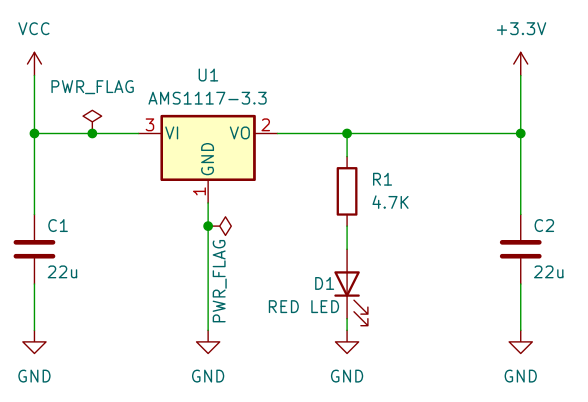
\includegraphics[width=.4\textwidth]{spannungsRegulierung}
    \caption{Spannungsregulierung des Erweiterungsmoduls}
    \label{fig:spannungsRegulierung}
\end{figure}

\subsubsection{ESP32 Programmierlogik}
Mittels einer seriellen Verbindung zwischen dem Entwicklercomputer und dem Mikrocontroller wird der ESP32-Mikcrontroller programmiert. Da jedoch heutzutage wenige Rechner eine serielle Buchse besitzen, gibt es grundlegend zwei Möglichkeiten den ESP32 zu programmieren. Die erste Möglichkeit ist, ein USB-zu-Seriell-Programmiergerät zu verwenden, womit der Entwicklercomputer mittels USB die Programmierung durchführen kann. Die zweite Möglichkeit ist, auf der eigenentwickelten Platine ein USB-zu-Seriell-Converter \ac{IC} zu integrieren, womit direkt die Programmierung des ESP32 mittels USB erfolgen kann. Jedoch entstehen bei dieser Methode zusätzliche Kosten und es wird wichtiger Platz auf der Platine verschwendet, da das Erweiterungsmodul nur einmal nach der Bestückung der Platine programmiert werden muss. Aus diesen genannten Einschränkungen wird die erste Möglichkeit zur Programmierung des ESP32 verwendet.

Damit der ESP32 für die Programmierung automatisch in den benötigten Programmiermodus schaltet, hat die verfügbare ESP32-Programmiersoftware des Herstellers einen fest definierten Programmierablauf.  Der Programmierablauf verwendet, dafür zwei vorhandene Statusleitungen der seriellen Verbindung. Zum einen die \textit{Data Terminal Ready}-Leitung und zum anderen die \textit{Request To Send}-Leitung. Zusätzlich zu den verwendeten Statusleitungen werden noch zwei Transistoren, angeordnet wie in Abbildung \ref{fig:autoFlash} zu sehen, auf der Erweiterungsmodulplatine benötigt. Mittels dieser Schaltung werden die Kontakte \textit{EN} und \textit{Boot} des ESP32 zu Beginn der Programmierung passend beschalten. Der Kontakt \textit{EN} am ESP32 wird verwendet, um den ESP32 lauffähig zu betreiben (Pegel von 3,3~V) oder die Ausführung von Programmen auf dem ESP32 (Pegel von 0~V) zu verhindern. Mit dem Kontakt \textit{Boot} kann während des Starts des ESP32 festgelegt werden, ob der normale Ausführungsmodus (Pegel von 3,3~V) oder der Programmiermodus (Pegel von 0~V) gestartet werden soll. Zusätzlich muss bei der Programmierung beachtet werden, dass der maximale Spannungspegel der seriellen Verbindung bei 3,3~V liegen muss. \cite{espFlashTool}

\begin{figure}[h]
    \centering
    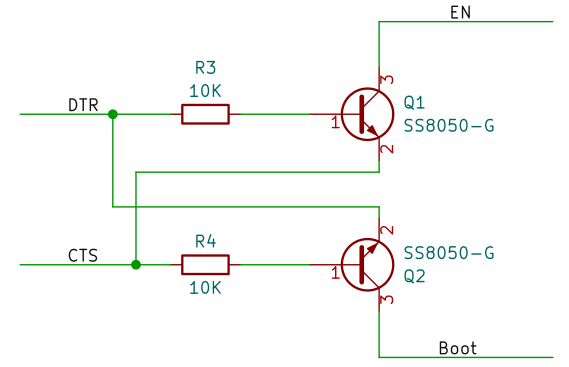
\includegraphics[width=.4\textwidth]{autoFlash}
    \caption{ESP32 Programmierlogik}
    \label{fig:autoFlash}
\end{figure}

\subsubsection{Tastenentprellung}
Zu Beginn der Betätigung eines Taster entstehen immer Schwingungen zwischen der Massespannung und der Betriebsspannung, was zur fehlerhaften Auswertung mittels eines Mikrocontrollers führt. Um dieses ungewollte Verhalten zu minimieren, beziehungsweise zu verhindern, sollten Tasten entprellt werden. Eine einfache Methode ist die Entprellung mittels Hardwarekomponenten, wie in Abbildung \ref{fig:buttonDebounce} zu sehen ist. Das Hauptelement zur Entprellung ist dabei der parallel zum Taster platzierte Kondensator \cite{debounceButton}. Damit bei Nichtbetätigung des Tasters eine Spannung von 3,3~V am ESP32-Kontakt anliegt, enthält jeder Kontakt des ESP32 einen internen Pull-Up Widerstand (45K Ohm). Eine Betätigung des Tasters zieht folgend die Spannung des ESP32-Kontakts auf eine Spannung von 0~V.

\begin{figure}[h]
    \centering
    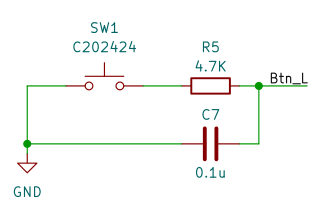
\includegraphics[width=.4\textwidth]{buttonDebounce}
    \caption{Hardwaretastenentprellung}
    \label{fig:buttonDebounce}
\end{figure}

Der Taster, welcher für den manuellen Start des Programmiermodis, auf der Platine des Erweiterungsmoduls vorhanden ist, darf jedoch nicht durch eine Hardwareschaltung entprellt werden. Da während der Aufladungsphase des Kondensators, sonst die Spannung am ESP32-Kontakt \textit{Boot} während des Starts nahe bei 0~V liegt und der ESP32 ungewollt im Programmiermodus gestartet wird.

\subsubsection{\acf{ESD}-Schutz}
\label{section:esdProtection}
Um zu vermeiden, dass durch elektrostatische Aufladung des Körpers das Erweiterungsmodul beschädigt wird, müssen die Kontakte des Erweiterungsmoduls geschützt werden. Der Schutz wird durch Zerner-Dioden, welche in Gegenrichtung mit 0~V verbunden sind, realisiert. Zu sehen ist die Schutzschaltung der Buchsenleiste des Erweiterungsmoduls in Abbildung \ref{fig:esdProtection}. Die Zerner-Dioden sind dabei so dimensioniert, das Spannungen größer 12~V (Versorgungsleitung) beziehungsweise größer 3,3~V (Datenleitung) über die Zener-Dioden Richtung 0~V geleitet werden.

\begin{figure}[h]
    \centering
    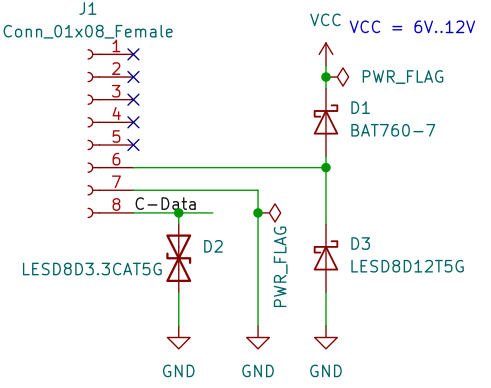
\includegraphics[width=.4\textwidth]{esdProtection}
    \caption{\ac{ESD}-Schutzschaltung}
    \label{fig:esdProtection}
\end{figure}

\subsection{Referenzschaltungen}
Zur Vermeidung von Fehlern während des Schaltungsentwurfs und zur Minimierung von Platinenproduktionsdurchgängen, bauen die Platinen des Erweiterungsmoduls auf Referenzdesigns, welche in der nachfolgenden Liste zu sehen sind, auf.

\begin{itemize}
    \item \acs{OLED}-Schaltplan von ShenZhen QDtech Co. LTD; Stand: 24.~Juli~2019
    \item ESP32\_DevKitc\_V4-Schaltplan von Espressif Systems (Shanghai Co., Ltd.); Stand: 7.~Juni~2018
    \item Produktspezifikation des OEL Display Module von Allvision technology Inc.; Version: B
\end{itemize}

\subsection{Weiterführende Informationen}

Alle Schaltpläne der Erweiterungsmodulplatinen sind im Anhang in den Abbildung \ref{fig:mainPCB}, \ref{fig:ioPCB} und  \ref{fig:connectorPCB} zu finden. Die vollständigen Platinenprojektdateien sind öffentlich unter folgenden Link auffindbar: \url{https://github.com/SimLinkModule/PCB}

Die Platinen sind dabei mit der kostenlosen Open Source Software KiCad \cite{aboutkicad} entwickelt worden und die Produktion und die Bestückung der meisten Elektronikkomenten fand durch das Unternehmen \href{https://jlcpcb.com/}{JLCPCB} statt.

\section{Gehäuseerstellung}
\label{section:caseImplementation}
Damit die entworfenen Platinen fest und kompakt im Modulschacht (Typ: Lite) der Fernsteuerung befestigt werden können, ist zusätzlich ein Kunststoffgehäuse entwickelt worden, welches mittels eines \ac{FDM}-3D-Druckers hergestellt werden kann. Alle benötigten Komponenten, des Gehäuses, sind im Anhang als Explosionszeichnung in Abbildung \ref{fig:shellPartsExplosion} zu sehen.

Der Fokus im Gehäuseentwurf liegt darin, das Gehäuse zu drucken, dass eine möglichst geringe Nachbearbeitung der Oberfläche nötig ist. Eine Nachbearbeitung, beim 3D-Druck mit dem \ac{FDM}-Verfahren, wird hauptsächlich an Oberflächen benötigt, welche mittels Stützstrukturen gedruckt werden. Um Stützstrukturen im Druck zu vermeiden, sollte auf Überhänge im Modell verzichtet werden. Diese Einschränkung geht aus dem \ac{FDM}-Verfahren hervor, da nur ausgehend vom Druckbrett des 3D-Druckers gedruckt werden kann. Falls jedoch nicht auf Überhänge verzichtet werden kann, gibt es zwei bekannte Möglichkeiten, um auf Stützstrukturen zu verzichten. Eine Möglichkeit ist das Modell in mehrere Teilmodelle aufzuteilen, welche einzeln ohne Stützstrukturen gedruckt werden können. Zu sehen ist dieses Verfahren in Abbildung \ref{fig:overhangCut}. Die zweite Möglichkeit ist, Stützstrukturen in das Modell zu integrieren. Diese Stützstrukturen, sollten wie in Abbildung \ref{fig:overhangStruct} zu sehen ist, einen Winkel zwischen 45 und 90 Grad zum Druckbrett haben.

\begin{figure}[h]
    \centering
    \includegraphics[width=.8\textwidth]{overhangCut}
    \caption{Modell mit Überhängen für den 3D-Druck vorbereiten}
    \label{fig:overhangCut}
\end{figure}

\begin{figure}[h]
    \centering
    \includegraphics[width=.5\textwidth]{overhangStruct}
    \caption{Modell mit Überhängen für den 3D-Druck vorbereiten}
    \label{fig:overhangStruct}
\end{figure}

Zur Befestigung aller Komponenten im Kunststoffgehäuse sind mehrere Gewindeeinsätze aus Messing integriert. Dies bietet den Vorteil, dass die einzelnen Komponenten des Erweiterungsmoduls mehrfach ein und ausgebaut werden können, da vorhandene integrierte Gewindegänge im Kunststoffgehäuse leicht überdreht und dadurch beschädigt werden können. Zu sehen sind alle benötigten Messinggewindeeinsätze des Gehäuses in Abbildung \ref{fig:pcbMounts}.

\begin{figure}[h]
    \centering
    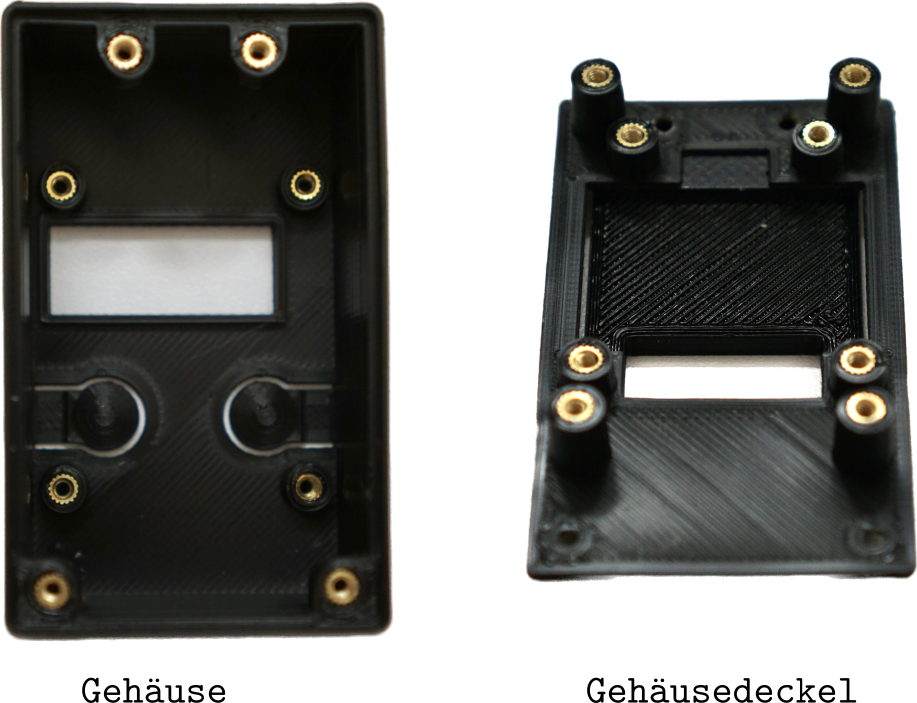
\includegraphics[width=.4\textwidth]{pcbMounts}
    \caption{Messing Gewindeeinsätze zur Befestigung der einzelnen Modulkomponenten}
    \label{fig:pcbMounts}
\end{figure}

Da der Gehäusedeckel, auf einer Seite Befestigungen für die Platinen hat und sich auf der gegenüberliegenden Seite die Schienen des Modulschachts befinden, ist dieses 3D-Modell in zwei Teilmodelle aufgeteilt. Dies ist nötig, um sowohl ohne Stützstrukturen auszukommen als auch die filigranen Schienen mit einer guten Qualität drucken zu können. Für eine höhere Stabilität des Gehäusedeckels sollten die Teilmodelle nach dem Druck mittels Kleber verbunden werden.

Damit die Platine mit der Modulbuchse im Gehäuse befestigt werden kann, werden zusätzlich gedruckte Kunststoffhalterungen benötigt. Dies ist nötig, da die Platine sehr nah an der Gehäuseaußenkante liegen muss, um eine Verbindung mit dem Stecker der Fernsteuerung herstellen zu können. Zu sehen sind die eingebauten Platinen in Abbildung \ref{fig:moduleAssembly}, sowie die Position der Modulbuchse für die Verbindung mit der Multikopterfernsteuerung.

\begin{figure}[h]
    \centering
    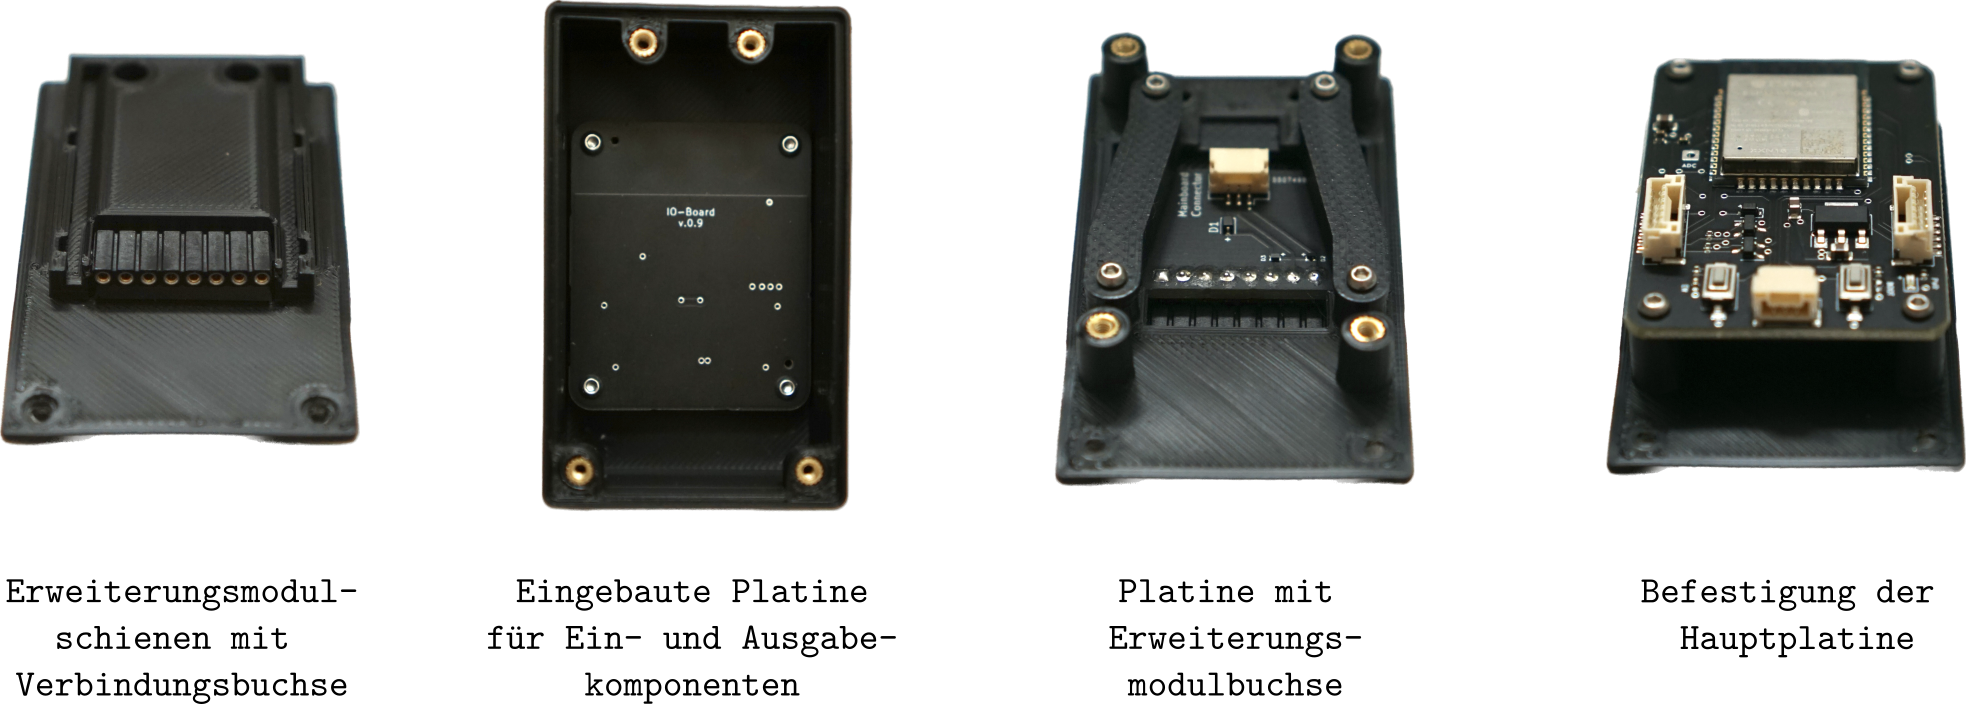
\includegraphics[width=1\textwidth]{moduleAssembly}
    \caption{Eingebaute Platinen im Gehäuse}
    \label{fig:moduleAssembly}
\end{figure}

Zum Schutz und zur Vergrößerung der Tasterdruckfläche der Taster der Eingabe- und Ausgabeplatine, ist ein integrierter Tasterschutz im Gehäuse vorhanden. Dieser Schutz und das Erweiterungsmodulgehäuse bilden dabei ein Bauteil, wodurch kein zusätzlicher Zusammenbau benötigt wird. Jedoch muss dafür das Verbindungsstück zwischen Tasterschutz und dem Gehäuse flexibel entworfen werden. Dies ist möglich, indem die Schichtdicke des Verbindungsstücks verringert wird, damit der Kunststoff biegsam wird. Zu sehen ist der Tasterschutz mit Verbindungsstück in Abbildung \ref{fig:buttonShell}. Zusätzlich ist in Abbildung \ref{fig:buttonShell} zu sehen, dass ein konischer Zylinder auf dem Tasterschutz vorhanden ist, womit die Tastendruckfläche vergrößert und die Lücke zwischen der befestigten Platine und dem Erweiterungsmodulgehäuse überbrückt wird.

\begin{figure}[h]
    \centering
    
\includegraphics[width=0.6\textwidth]{buttonShell}
    \caption{Tasterschutz für Taster der Platine}
    \label{fig:buttonShell}
\end{figure}

\subsection{Weiterführende Informationen}
In Abbildung \ref{fig:moduleComplete} ist das vollständig montierte Gehäuse mit eingebauten Platinen zu sehen.

\begin{figure}[h]
    \centering
    \includegraphics[width=0.3\textwidth]{moduleComplete}
    \caption{Zusammengebautes Erweiterungsmodul}
    \label{fig:moduleComplete}
\end{figure}

Der Entwurf des Gehäuses fand in der kostenlosen und Open Source Software OpenSCAD \cite{aboutOpenScad} statt. Die zugehörigen Projektdateien sind öffentlich unter folgenden Link auffindbar: \url{https://github.com/SimLinkModule/Shell}